\chapter{Introduction}
\label{ch:chap1}

%----------------------------------------------------------------------------------------

\begin{chapquote}{Michel Foucault, \textit{The Truth is in the Future}.}
All human behaviour is scheduled and programmed through rationality. There is a logic of institutions and in behaviour and in political relations. In even the most violent ones there is a rationality. What is most dangerous in violence is its rationality. Of course violence itself is terrible. But the deepest root of violence and its permanence come out of the form of the rationality we use. The idea had been that if we live in the world of reason, we can get rid of violence. This is quite wrong. Between violence and rationality there is no incompatibility.
\end{chapquote}

On 18th February 2001, Brazil's richest state was brought to a halt. In one ordinary Sunday afternoon, the \textit{Primeiro Comando da Capital}\footnote{Portuguese for ``First Command of the Capital'', the capital being the city of S\~{a}o Paulo. All abbreviations mentioned in this text, alongside their respective translations into English, are listed on page \pageref{sec:acronyms}.} (PCC hereafter) unexpectedly challenged the government forces and took over 29 prisons across the state of S\~{a}o Paulo \citep[208]{biondi2007relacoes}. According to official estimates, about 25,000 prisoners joined the rebellion, and in a single penitentiary, 8,000 inmates held more than 7,000 civilians as hostages, amongst them 1,750 children \citep[]{terra2001rebeliao}. The convicts protested against the transference of PCC leaders from the capital to the countryside. To organise what became known as ``the megarebellion'', they had been using smuggled mobile phones \citep[]{montandon2012sistema}. Heavily-armed government troops later stormed the prisons, and after hours of negotiations and the eventual use of lethal force (5 inmates were killed), the criminal organisation was finally contained. Nevertheless, the damage to the government's reputation had already been done. It was clear to everyone -- the media, public officials, citizens -- that the PCC was a social force not to be ignored. As summarised by \citet[387]{amorim2003cv}, in 2001, the PCC ``[\dots] publicly declared their hegemony over the prison system in S\~{a}o Paulo. A hegemony backed up by the magnitude of the rebellion itself [\dots].'' 

Five years later, the PCC performed yet another show of force. Between May and June 2006, the \textit{Comando} organised a series of attacks in no less than 82 prisons, 10 of them in other states. The violence also spread outside the prison walls. According to the Secretary of Public Security (SSP), PCC-affiliated members burned 82 buses, bombed 17 bank branches, killed 46 and wounded 78 police officers and penitentiary agents in 280 attacks to public buildings in the city of S\~{a}o Paulo alone \citep[]{folha2006rebeliao, terra2008rebeliao}. 

\begin{center}
\begin{figure}[bth]
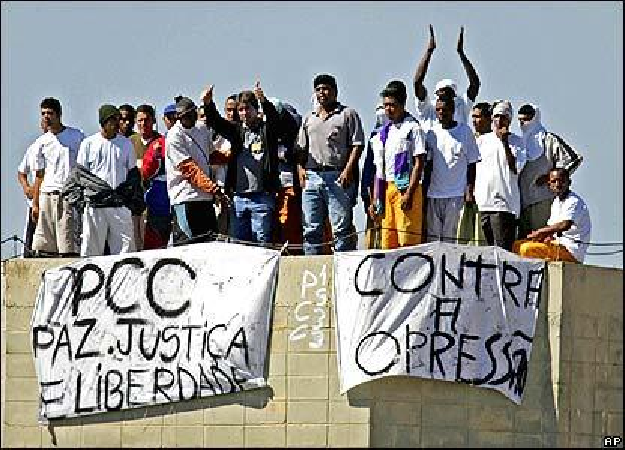
\includegraphics[height = 8cm, width = 1\linewidth]{gfx/fig1}
\caption[PCC Rebellion in 2006]{PCC Rebellion in 2006\footnotemark}
\label{fig:fig1}
\end{figure}
\end{center}

\footnotetext{Source: Associated Press. The banners read ``PCC, peace, justice and freedom'', and ``against oppression''. Regarding the 1533 written on the wall, the letter P is the 15th and C is the 3rd in the Brazilian alphabet, whereby 1533 means PCC. Except otherwise noted, all translations from Portuguese to English are my own.} The two rebellions have led to heated debates about the role of prison reform in the society \citep[323]{dias2009guerra}. Brazil's incarcerated population has skyrocketed in the last decades, and S\~{a}o Paulo provides perhaps the best example of such steady increase. The country currently has the fourth largest incarceration population in the world with around 574,000 prisoners\footnote{This number is only smaller than those of the United States (2.2 million inmates), China (1.6 million) and Russia (740,000) \citep{agenciabrasil2014prisaobrasil}.}. S\~{a}o Paulo alone holds around 200,000 convicts (35\% of the total) and adds another 15,000 inmates to the official statistics every year \citep{brasildefato2013numeropresos}. The trend can be seen in \autoref{fig:fig2} below. The massive growth in incarceration rates has created serious problems to the Brazilian prison system: overcrowding, staff shortage, and inadequate legal services, sanitation and health care present in virtually every penitentiary of the country \citep[275]{darke2013inmate}.

\begin{center}
\begin{figure}[bth]
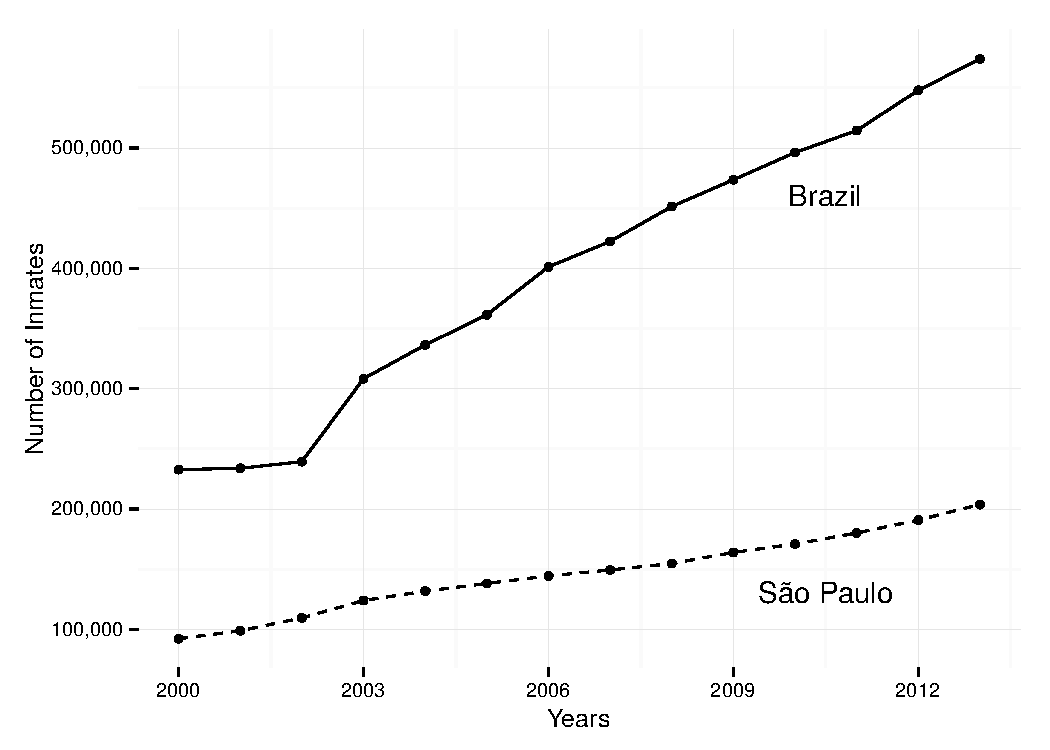
\includegraphics[height = 8cm, width = 1\linewidth]{gfx/fig2}
\caption[Prison Population (2000--2013)]{Prison Population (2000--2013)\footnotemark}
\label{fig:fig2}
\end{figure}
\end{center}

\footnotetext{Source: Own authorship with data provided by the Brazilian Ministry of Justice. Stable links: \href{http://bit.ly/1rImlPE}{http://bit.ly/1rImlPE} and \href{http://bit.ly/1ixhY8z}{http://bit.ly/1ixhY8z} [Access: 23th April 2014]. All graphs displayed in this thesis were created with \texttt{R} statistical language version 3.1.0 \citep{rstats} and the \texttt{ggplot2} package version 0.9.3.1 \citep{ggplot2}. Reproducible code for the figures are included in the \autoref{sec:appendix}.} Furthermore, as in other parts of the country \citep{zaluar1999debate}, the vast majority of prisoners in S\~{a}o Paulo are black and from low social strata \citep[16]{adorno2007organized}, groups with few economic opportunities apart from those offered by illicit markets\footnote{Brazil was a slave country until 1889, and racial prejudice has never been absent in the country. While blacks currently comprise 51\% of the Brazilian population \citep{secretariaassuntos2012populacaonegra}, they make 66\% of homicide victims and 65\% of the total number of convicts in the country \citep{waiselfisz2012mapa}. As described by \citet[1]{adorno1996racismo}, ``[\dots] crime is not exclusive to the black population, but punishment seems to be.''}. In this regard, prison gangs are not only important for protection, but also for being able to reduce the ``income loss'' suffered by an individual if he is put behind bars. The PCC was explicitly structured around this principle: its internal statute clearly declares that ``[\dots] those who are in liberty [should contribute] to the brothers inside prisons [PCC members] through lawyers, money, help to family members and prison outbreak operations'' \citep{folha2001estatutopcc}. By giving economic incentives to other inmates, the PCC can expand their cadres and increase the general welfare of the inmates. In a region where inequality is rampant and the state has thus far failed to properly address the issue of poverty \citep{chiavegatto2012cause, marques2012opportunities}, the fact that the PCC currently provides food supplies, financial assistance, medicines, private health care, and legal advice \citep{defesanet2012estatutopcc} makes the organisation notably attractive for a large number of inmates. 

It has also been noted that the PCC significantly contributed to the reduction in violence within S\~{a}o Paulo's prison system. At least since the mid-2000s, the group has been able to emerge as an undisputed mediator and solve conflicts between inmates. \citet[83]{dias2009ocupando} affirms that ``[\dots] when unable to constitute a universal source of regulation, the official law leaves gaps which are filled by informal instances -- such as the Primeiro Comando da Capital (PCC), in the prisons of S\~{a}o Paulo.'' The gang has implemented informal courts that resemble state institutions, and those ``debates'' -- how such illegal tribunals are called\footnote{The original term is spelt the same way in Portuguese, \textit{debates} \citep[3]{feltran2012metodos}.} -- have progressively replaced other forms of ``popular justice'' such as lynchings and hiring of target killers \citep[3]{feltran2012metodos}. Moreover, the \textit{Comando} has developed a series of assertive ways to verbally terrorise inmates. Since the PCC's threats are credible, such meetings with actual or potential undisciplined members are effective deterrence factors\footnote{The practice is known within and outside PCC circles as \textit{dar um psicol\'{o}gico}, ``to put psychological [pressure]'' \citep{marques2010liderancca}.}.

The rise of the PCC has also brought other positive changes to public security. The city of S\~{a}o Paulo, capital of the state of the same name, was knowingly one of the most violent places in the world. Nevertheless, S\~{a}o Paulo has experienced a drastic reduction in homicides over the past years. A number of authors argue that the establishment of the PCC as the city's (and the state's) major drug gang has accounted for most of the decline in murders in the metropolis. \cite{biondi2010junto} and \cite{dias2011pulverizaccao}, for instance, note that the PCC has instituted a policy that explicitly forbids the use of lethal violence as a means to settle disputes between members and severely punishes those who refuse to abide by that rule \citep{jozino2004cobras}. Since poor young males have the highest risk of being both victims of murder in S\~{a}o Paulo and members of the PCC, the correlation between the emergence of the cartel and the drop in homicide rates seems plausible. \autoref{fig:fig3} shows the evolution of murder rates in the city of S\~{a}o Paulo. 


%From 2000 to 2007, the number of murders declined from 5,979 to 1,311 (-78\%), and S\~{a}o Paulo's poorest districts have seen even larger declines in murder rates. Homicides in Cap\~{a}o Redondo declined from 203 in 2002 to 23 in 2007; in Itaquera, from 140 in 2001 to 20 in 2007; in Cidade Tiradentes, from 195 in 2000 to 24 in 2007; and in Jardim \^{A}ngela there were 53 homicides in 2007, down from 277 in 2001. 

\begin{center}
\begin{figure}[bth!]
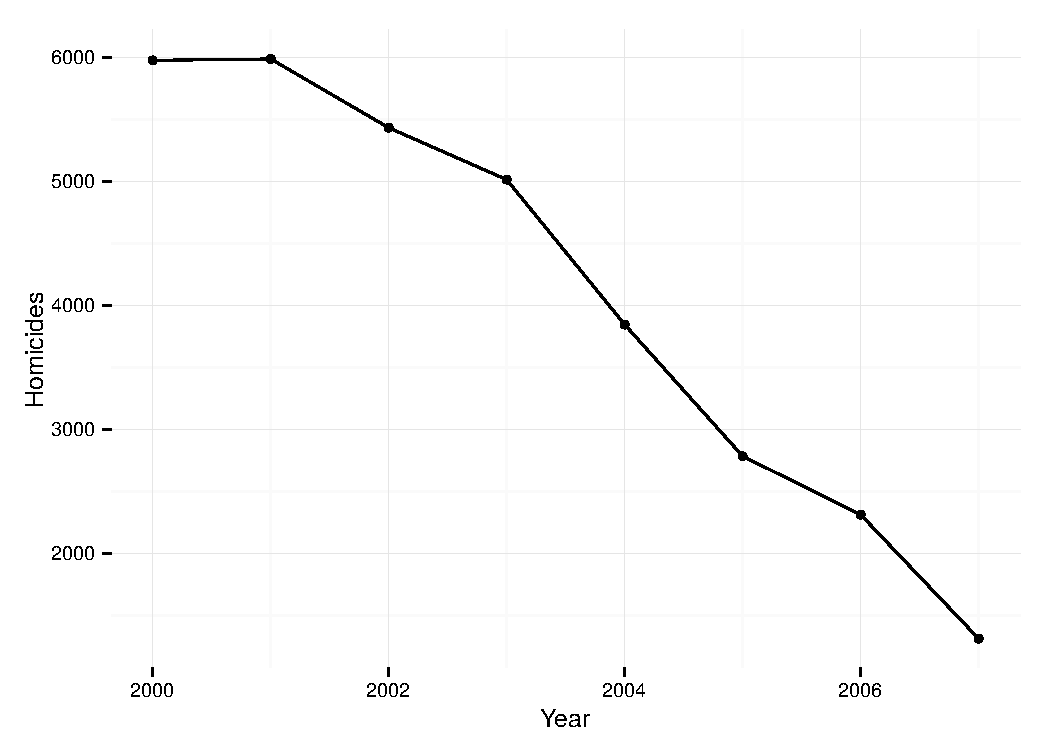
\includegraphics[height = 8cm, width = 1\linewidth]{gfx/fig3}
\caption[Homicides in S\~{a}o Paulo (2000--2007)]{Homicides in S\~{a}o Paulo (2000--2007)\footnotemark}
\label{fig:fig3}
\end{figure}
\end{center}

\footnotetext{Source: Own authorship. Data collected by the Centre for the Study of Violence at the University of S\~{a}o Paulo. Stable link: \href{http://bit.ly/Sg7qjB}{http://bit.ly/Sg7qjB} [Access: 24th March 2014].} %The reduction of violence in poor areas have also lent legitimacy to the PCC. The cartel can now enjoy greater support from the extended families of the inmates, many of them who directly benefited from the lowering of homicide rates \citep{feltran2008legitimo, feltran2012metodos}.

Curiously, the PCC has managed to accomplish all those goals while representing \textit{less than 3\%} of S\~{a}o Paulo's inmate population \citep[]{bbc2013pcc, veja2013crescimentopcc}. The task is indeed impressive if one keeps in mind that criminals face enormous challenges when trying to provide private governance \citep{sheptycki2003governance}. Given the constant fear of being arrested by the police \citep{williams2002cooperation}, criminals encounter several problems to identify their peers and communicate with each other \citep[xii]{gambetta2009codes}. Also, as a result of the inherently violent nature of many illegal activities, attempts to establish bonds of trust between criminals are rare and likely to fail \citep{liebling2012social, von2004organized}. Due to these obstacles, criminal networks are an intriguing object of study for those interested in cooperation issues and the role of violence, incentives and signals as credible commitments in social groups \citep{campana2013cooperation, densley2012street, freeman1994crime}.

This poses two clear questions that so far have not been addressed by the specialised literature on the PCC. First, why is not \textit{every} detainee a PCC member? Since the PCC is able to considerably ameliorate prison conditions, why would someone prefer \textit{not} to join the gang? ``Going alone'' seems to be an irrational strategy to all inmates, so why would they adopt it? Second, how can the PCC find a ``competent'' criminal to join its ranks in such a violent, uncertain environment as the prison? As any other organisation or firm, the PCC knows that ``qualified candidates'' are a scarce resource, and the group wants to select qualified mobsters and reject bad ones. But how can the gang do so if criminals have strong incentives to hide their intentions and lie about their skills? 

%Given the clear importance of the PCC in Brazil's current history, it is surprising that the topic has attracted such a limited number of researchers. \citet[365]{dias2011pulverizaccao} notes that while there is a significant number of writings focused on the judicial dimension of organised crime, the literature analysing empirical aspects of criminal institutions is still comparatively small. Apart from a few books written by investigative journalists \citep{amorim2003cv, jozino2004cobras, souza2007pcc}, and some fieldwork studies produced by anthropologists and sociologists \citep{biondi2010junto, dias2009guerra, dias2011pulverizaccao, marques2010liderancca}, no analytical work has ever been written on the group. In this sense, political scientists could contribute to this debate not only by offering a more general theory derived from the findings presented in the literature, but also by using techniques which have so not been employed to analyse the organised crime in S\~{a}o Paulo. 

In the present thesis, I develop a formal model to address these  lacunae in the recent literature. Game theory is a useful tool to evaluate deductive logic and test causal mechanisms, specially in situations where first-hand information is either unavailable or too risky to obtain. However, while those methods are now widely employed in international relations and comparative politics  \citep[e.g.][]{de1999institutional, fearon1995rationalist, mccarty2007political}, their use is still notably limited in criminal studies. With noteworthy exceptions \citep[]{dixit2011game, lessing2014cddrl}, formal theorists have so far largely ignored prison gangs. With regards to the PCC, there is not a single study that uses formal modelling to evaluate the operations of the cartel, even though some of the topics related to the organisation could be translated into mathematical terms. This work aims to partially fill this gap.

In \autoref{ch:chap2} I offer a brief review of the recent literature on prison culture and gangs, emphasising the Brazilian contributions to the topic. \hyperlink{page.19}{Chapter 3} presents a short history of the Primeiro Comando da Capital, which to the best of my knowledge has not yet been published in the English language. In \autoref{ch:chap4} I develop a simple formal model discussing under what condition inmates would decide to join the criminal organisation and how the PCC is able to successfully select potential candidates. Based upon the rational theory of crime and on qualitative evidence, I intend to present a general framework to understand the problems of individual choice regarding a criminal organisation, and decision-making under conditions of extreme uncertainty. Both analyses are knowingly modest, but they represent new contributions to the field.

%% Comment this last paragraph


% \citep[e.g.][]{bhavnani2006ethnic, bhavnani2000localized, de1999institutional, epstein2002modeling, mccarty2007political}
